\documentclass[conference]{IEEEtran}

\usepackage[utf8]{inputenc}
\usepackage[T1]{fontenc}
\usepackage{silence}\WarningsOff[latexfont]

\usepackage{amsmath}

\RequirePackage{tikz}[2010/10/13]
\usetikzlibrary{arrows,automata,calc,intersections,patterns,decorations.pathmorphing,decorations.pathreplacing}

\usepackage{graphicx}
\usepackage{cite}
\usepackage{url}
\usepackage[caption=false,font=footnotesize]{subfig}
\usepackage[binary-units,per-mode=symbol]{siunitx}
\sisetup{list-final-separator = {, and }}
\usepackage{booktabs}
\usepackage{pifont}
\usepackage{microtype}
\usepackage{textcomp}
\usepackage[american]{babel}
\usepackage[noabbrev,capitalise]{cleveref}
\usepackage{xspace}
\usepackage{hyphenat}
\usepackage[draft,inline,nomargin,index]{fixme}
\fxsetup{theme=color}
\usepackage{grffile}
\usepackage{xfrac}
\usepackage{multirow}
\RequirePackage{xstring}
\RequirePackage{xparse}
\RequirePackage[index=true]{acro}

\NewDocumentCommand\acrodef{mO{#1}mG{}}{\DeclareAcronym{#1}{short={#2}, long={#3}, #4}}
\NewDocumentCommand\acused{m}{\acuse{#1}}

\usepackage{upquote}

\acrodef{MAC}{Medium Access Control}
\acrodef{RV}{Random Variable}
\acrodef{MC}{Markov Chain}
\acrodef{CTMC}{Continuous Time Markov Chain}

\begin{document}

\title{Aloha Markovian Model}
\author{
	\IEEEauthorblockN{Davide Pedranz, Mat. number 189295}
	\texttt{davide.pedranz@studenti.unitn.it}
}

\maketitle

\begin{abstract}
Models are powerful mathematical tools that allow a very quick and efficient system analysis.
They can be used to analyze protocols and systems before building them or to confirm the results of simulations.
In this assignment, we will build a Markovian Model for the Aloha MAC protocol and compare it with the results of the simulator. 
\end{abstract}

\acresetall

\section{Introduction}
\label{sec:introduction}

Models are powerful and widely used tools to analyze, compare and evaluate the performances of a system.
Together with simulations, they allow to take the right decisions in the design and construction of a system and guarantee that it behaves as expected.
Models predict the behaviour of a system as a function of some parameters, allowing a very cheap and effective ``what-if'' analysis.

In this assignment, we will build and present a Markovian Model for the Aloha \ac{MAC} protocol.
We will briefly discuss the behaviour of Aloha. Then, we will present the assumptions we started from and show how we build and refined the model step-by-step.
Finally, we will compare the model's predictions with the the simulator's results.

\section{Aloha}
\label{sec:aloha}

A \ac{MAC} protocol defines how stations access a shared channel in order to transmit packets to the others.
Aloha is a very simple \ac{MAC} protocol developed by Norman Abramson and his colleagues at the University of Hawaii in the 1970s to realize a broadcasting communication between nodes spread on different islands of the archipelago.

The behaviour of Aloha is the following: when a packet arrives to the station, it is immediately transmitted.
When a station is idle, it listens for incoming packets.
If new packets to transmit arrive while the station is already transmitting, receiving or processing another packet, they will be queued and will be processed as soon as the station finishes the current action.
Aloha does not guarantee to deliver a packet.
If multiple packets are transmitted at the same time by different stations, they are very likely to collide and be unrecognizable.
In other words, there is no guarantee that a packet will be correctly received by the other stations.

\section{Aloha Analysis}
\label{sec:theoretical_aloha}

A theoretical analysis of the Aloha protocol has been proposed by Tanenbaum in 2003 \cite{tanenbaum2003computernetworks}.
The model is derived from the analysis of packets collisions assuming that packets follow a Poisson process.
The predicted throughput is computed as:
\begin{equation*}
    throughput = G \cdot e^{-2G} \cdot r\,,
\end{equation*}
where $G$ is the normalized load, i.e. the average number of packets transmitted for each unit of time, and $r$ denotes transmission rate of each station \cite{wiki:aloha}.
$G$ can be computed as the total offered load over the transmission rate:
\begin{equation*}
    G = \frac{load}{r}\,.
\end{equation*}

\section{Markovian Models}
\label{sec:markov}

A stochastic process is an ordered collection of random variables:
\begin{equation*}
    \{X(t,s) \,|\, t \in T, s \in S\},
\end{equation*}

where $t$ is the index (or time) of the process and $s$ the space of possible values that the \ac{RV} can assume.

The process $X$ is a Markov Process if:
\begin{equation*}
    \begin{gathered}
        P[X(t_{n+1}) \leq x_{n+1} \,|\, X(t_n) = x_n, ... , X(t_0) = x_0] = \\
        = P[X(t_{n+1}) \leq x_{n+1} \,|\, X(t_n) = x_n].
    \end{gathered}
\end{equation*}

for $t_0 < t_1 < ... < t_n < t_{n+1}$.
In other words, the value of the \ac{RV} $X(t_{n+1})$ depends only on the value of the previous \ac{RV} $X(t_n)$.
The evolution of the process if fully described in its current state and is independent on its history.

A Markov Process with discrete space $S$ can be modelled as a \ac{MC}.
A \ac{MC} is a directed graph, where the nodes indicate the state of the process and edges indicate transitions between states.
Each edge is associated with some transition rate, usually represented as the graph matrix that completely characterize the process.
On certain conditions, the \ac{MC} admits a steady state, i.e. each state has a given probability which is independent on the initial state of the process.
If it exists, the steady states solution is given by the solution of a simple system of linear equations, as showed in \cref{sec:first_model}.

\section{Assumptions}
\label{sec:assumptions}

The models we present assume a single shared channel and stations $n$ stations, all in the communication range of each other.
Packets have exponential interarrival time of mean $\lambda^{-1}$.
$\mu$ indicates the average number of packets that exit the channel per unit of time

To keep the model simple, we assume an exponential distribution with mean $s=746\, byte$ for the packets size.
Each station transmit at a data rate $r$ of $8\, Mbps$.
We assume that all packets are corrupted in case of collisions, i.e. when there is more than one packet on the channel.

\section{First Model}
\label{sec:first_model}

The first model uses a \ac{CTMC} to represent the state of the channel.
Each node indicate the number of packets currently on the channel.
At the beginning there are zero packets.
At any moment, all station have an equal probability to start to transmit at any given moment: the transition from state $0$ to state $1$ has a rate of $n \lambda$.
If there is $1$ packet on the channel, one station is already transmitting and it will not be able to transmit another packet at the same time.
Thus, the rate to move from state $1$ to state $2$ is given by $(n-1) \lambda$.
For the same reason, the transition rate from state $k$ to $k+1$ is given by $(n - k) \lambda$.

Each packet needs some time to be transmitted.
Since we assumed an exponential distribution for the sizes, we define $\mu$ as follows:
\begin{equation*}
    \mu = \frac{1}{t_{TX}}
    = \Big( \frac{s}{r} \Big) ^ {-1}
    = \frac{r}{s},
\end{equation*}

where $t_{TX}$ denotes the transmission time for one averaged sized packet.

\begin{figure}[t!]
    \centering
    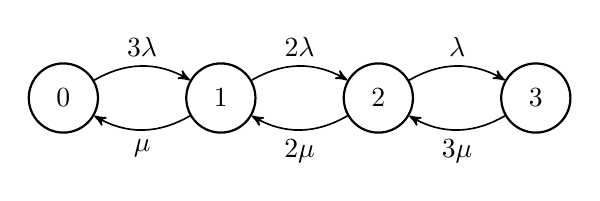
\begin{tikzpicture}[->, >=stealth', auto, semithick, node distance=2cm]
        \tikzstyle{every state}=[fill=white,draw=black,thick,text=black,scale=1]
        
        \node[state]    (0)                 {$0$};
        \node[state]    (1)[right of=0]     {$1$};
        \node[state]    (2)[right of=1]     {$2$};
        \node[state]    (3)[right of=2]     {$3$};
        
        \path
            (0) edge[bend left]    node{$3\lambda$}     (1)
            (1) edge[bend left]    node{$2\lambda$}     (2)
            (2) edge[bend left]    node{$\lambda$}      (3)
            (3) edge[bend left]    node{$3\mu$}         (2)
            (2) edge[bend left]    node{$2\mu$}         (1)
            (1) edge[bend left]    node{$\mu$}          (0)
        ;
    \end{tikzpicture}
    \caption{Markov Chain that represent the first model for $3$ stations. The state represent the number of nodes on the channel.}
    \label{fig:simple}
\end{figure}

Since the \ac{CTMC} is time-homogeneous and has only recurrent-positive states, it admits a steady state solution $\pi$ that can be computed as:
\begin{equation*}
    \begin{cases}
        \sum_{i=0}^{n} \pi_i = 1 \\[0.5em]
        \pi Q = 0
    \end{cases}
\end{equation*}

$Q = [q_{ij}]$ is the infinitesimal generator matrix that represent the transitions rate from state $i$ to $j$ of the chain.
For any \ac{CTMC}, the diagonal $q_{ii}$ of the matrix $Q$ is defined as:

\begin{equation*}
    q_{ii} = - \!\!\! \sum_{j = 0, j \neq i}^{\infty} q_{ij}.
\end{equation*}

For $n=3$ showed in \cref{fig:simple} we have:
\begin{equation*}
Q =
\begin{bmatrix}
    -3\lambda   & 3\lambda            & 0                   & 0         \\
    \mu         & (-2\lambda - \mu)   & 2\lambda            & 0         \\
    0           & 2\mu                & (-\lambda - 2\mu)   & \lambda   \\
    0           & 0                   & 3\mu                & -3\mu
\end{bmatrix}
\end{equation*}
\begin{equation*}
    \begin{cases}
        \pi_0 + \pi_1 + \pi_2 + \pi_3 = 1 \\
        -3\lambda\pi_0 + \mu\pi_1 = 0 \\
        3\lambda\pi_0 + (-\lambda-2\mu) + 2\mu\pi_2 = 0 \\
        2\lambda\pi_1 + (-\lambda-2\mu)\pi_2 + 3\mu\pi_3 = 0 \\
        \lambda\pi_2 - 3\mu\pi_3 = 0
    \end{cases}
\end{equation*}

which holds the solution:
\begin{equation*}
    \begin{aligned}[l]
        \pi_0 = \frac{\mu^3}{(\lambda + \mu)^3}, \\[1em]
        \pi_1 = \frac{3\lambda\mu^2}{(\lambda + \mu)^3}, \\
    \end{aligned}
    \;\;\;\;\;
    \begin{aligned}[l]
        \pi_2 = \frac{3\lambda^2\mu}{(\lambda + \mu)^3}, \\[1em]
        \pi_3 = \frac{\lambda^3}{(\lambda + \mu)^3}.
    \end{aligned}
\end{equation*}

It is easy to show that the solution of this model for an arbitrary number of stations $n$ is given by:
\begin{equation*}
    \pi_i = \frac{\binom{n}{i} \lambda^i \mu^{n-i}}{(\lambda + \mu)^n}.
\end{equation*}

We are interested in the probability $\pi_1$ that there is only $1$ packet on the channel, since it is the only case when a packet can be transmitted without collisions.
Given $\pi_1$, we can compute the average throughput at the receiver as:
\begin{equation*}
    throughput = \pi_1 \cdot r \cdot \frac{n-1}{n}.
\end{equation*}

The term $\frac{n-1}{n}$ is given by the definition of throughput as the size of the received packets over the total size of emitted packets.
If we consider a single station, it receives packets from the other $n-1$ ones: the packets sent by itself are not counted in its throughput.

In a similar way, we can compute the collision rate as the probability of having $2$ or more packets in the air over the probability of at least $1$ packet:
\begin{equation*}
    collision\_rate = \frac{\sum_{i = 2}^{n} \pi_i}{\sum_{i = 1}^{n} \pi_i}.
\end{equation*}

The model does not consider the stations' packets queue: it assumes the stations to transmit each packet as soon as they receive it from the application.

\section{Second Model}
\label{sec:second_model}

In the previous model, state $1$ can be reached from either state $0$ or state $2$.
In the second case, the packet is very likely to be corrupted, since it was on the channel with another packet.
We shall refine the model to distinguish those cases.
We replace state $1$ with two new states: $1G$ ($1$ good) and $1B$ ($1$ bad).
State $1G$ can be reached only from state $0$, whereas state $1B$ can be reached only from state $2$.
\cref{fig:model2} shows the resulting \ac{MC} for $n=3$.

\begin{figure}[t!]
    \centering
    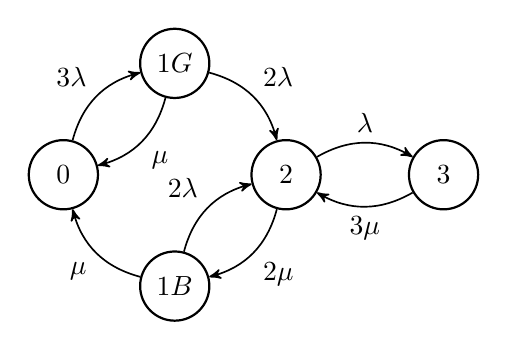
\begin{tikzpicture}[->, >=stealth', auto, semithick, node distance=2cm]
        \tikzstyle{every state}=[fill=white,draw=black,thick,text=black,scale=1]
        
        \node[state]    (0)                     {$0$};
        \node[state]    (G)[above right of=0]   {$1G$};
        \node[state]    (B)[below right of=0]   {$1B$};
        \node[state]    (2)[below right of=G]   {$2$};
        \node[state]    (3)[right of=2]         {$3$};
        
        \path
            (0) edge[bend left]    node{$3\lambda$}     (G)
            (G) edge[bend left]    node{$2\lambda$}     (2)
            (B) edge[bend left]    node{$2\lambda$}     (2)
            (2) edge[bend left]    node{$\lambda$}      (3)
            (3) edge[bend left]    node{$3\mu$}         (2)
            (2) edge[bend left]    node{$2\mu$}         (B)
            (B) edge[bend left]    node{$\mu$}          (0)
            (G) edge[bend left]    node{$\mu$}          (0)
        ;
    \end{tikzpicture}
    \caption{Markov Chain that represent the second model for $3$ stations. The state represent the number of nodes on the channel.}
    \label{fig:model2}
\end{figure}

As for the previous model, the \ac{CTMC} admits a steady state solution, which can be computed as follows:
\begin{equation*}
    \begin{cases}
        \pi_i = \frac{\binom{n}{i} \lambda^i \mu^{n-i}}{(\lambda + \mu)^n}, & \mbox{if } i \neq 1 \\[1em]
        \pi_{1G} = \frac{n \lambda \mu^n}{(\lambda + \mu)^n((n-1)\lambda + \mu)}, \\[1em]
        \pi_{1B} = \frac{n(n-1) \lambda^2 \mu^{n-1}}{(\lambda + \mu)^n((n-1)\lambda + \mu)}. \\
    \end{cases}
\end{equation*}

Note that $\pi_{1G} + \pi_{1B}$ equals to $\pi_1$ of the previous model.

Similarly to the previous model, throughout and collision rate are computed as follows:
\begin{equation*}
    throughput = \pi_{1G} \cdot r \cdot \frac{n-1}{n}\,,
\end{equation*}

\begin{equation*}
    collision\_rate = \frac{\pi_{1B} + \sum_{i = 2}^{n} \pi_i}{\pi_{1G} + \pi_{1B} + \sum_{i = 2}^{n} \pi_i}\,.
\end{equation*}

As for the first model, we assume that stations transmit packets as soon as they get them, so they do not have any queue.

\section{Comparison}
\label{sec:comparison}

The simulator has been run with $10$ stations.
All stations are in the communication range of each other, arranged on a ring of radius \SI{3}{\meter}, as shown in \cref {fig:topology}.

\begin{figure}[h!]
	\centering
	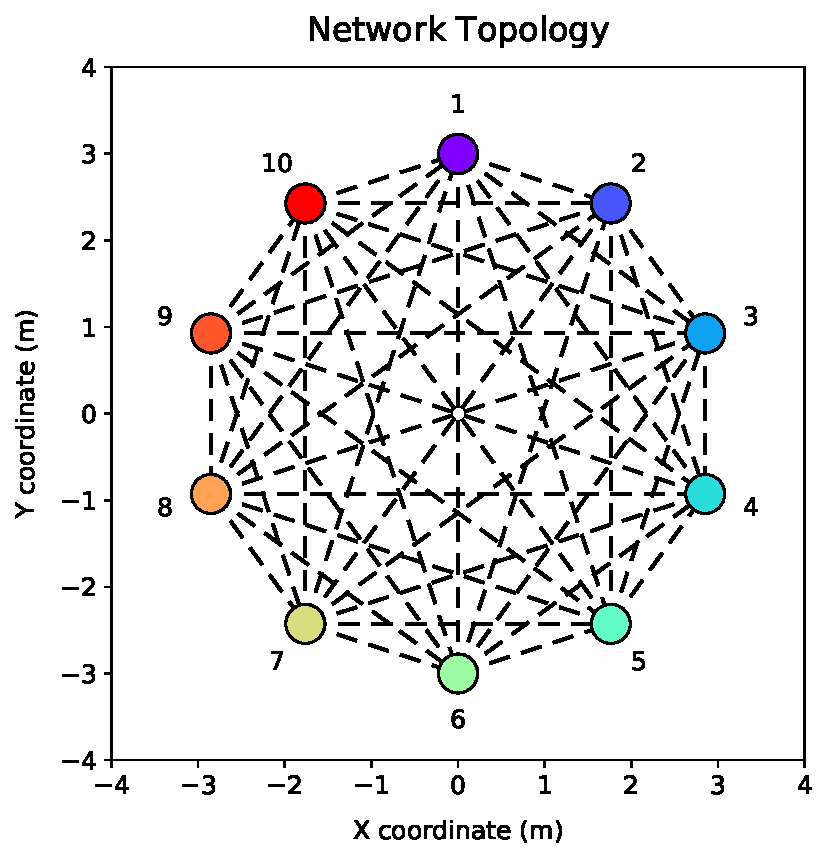
\includegraphics[width=.9\columnwidth]{figures/topology}
	\caption{Network topology used to run the simulations.}
	\label{fig:topology}
\end{figure}

\begin{figure}[t]
	\centering
	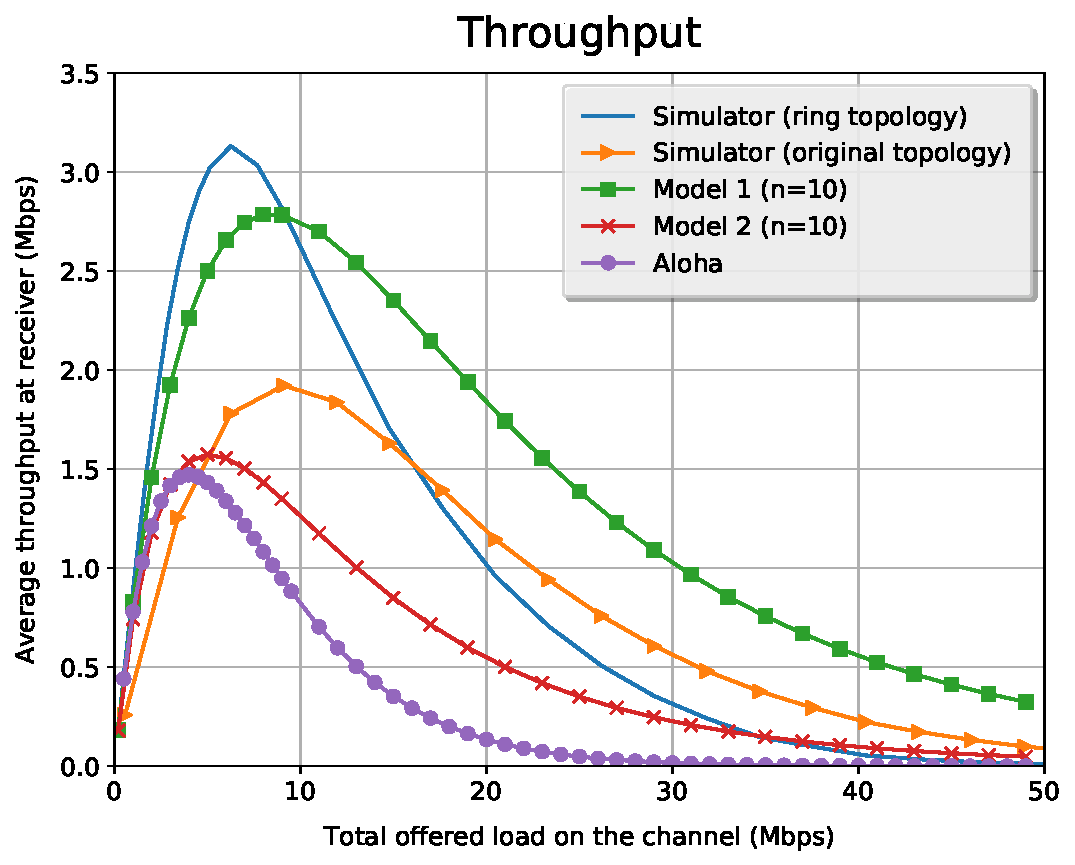
\includegraphics[width=.99\columnwidth]{figures/tr_10}
	\caption{The plot shows the throughput predicted by the different models for a network with 10 stations, compared with the theoretical model for Aloha and the simulator results.}
	\label{fig:tr_10}
\end{figure}

\cref{fig:tr_10} show the throughput predicted by the different models.
For very low loads, all models behave like the simulator.
For loads near the channel capacity ($8\, Mbps$), the simulator performs better than all models.
This is probably due to the behaviour of the simulated stations:
while a station is receiving a packet, it can not start to transmit.
This helps to avoid collisions and reach a higher throughput.
Models use means which do not take into account this particular behaviour.

The first model predicts a higher throughput than the second one, since it does not differentiate between the state with only one packet (1G) and the state with one packet that was corrupted by some collision (1B).

\cref{fig:tr_1g1b} compare the throughput predicted by the second model for different numbers of stations.
Regardless the number of station, the maximum throughput is before $10\,Mbps$, near the channel capacity.
With a small number of station, the maximum throughput is lower, but the throughput at high loads is slightly higher, due to the lower probability of collision.
With a high number of stations, the behaviour is closer to the theoretical model, but with a slightly higher throughput for all loads.

\begin{figure}[t]
	\centering
	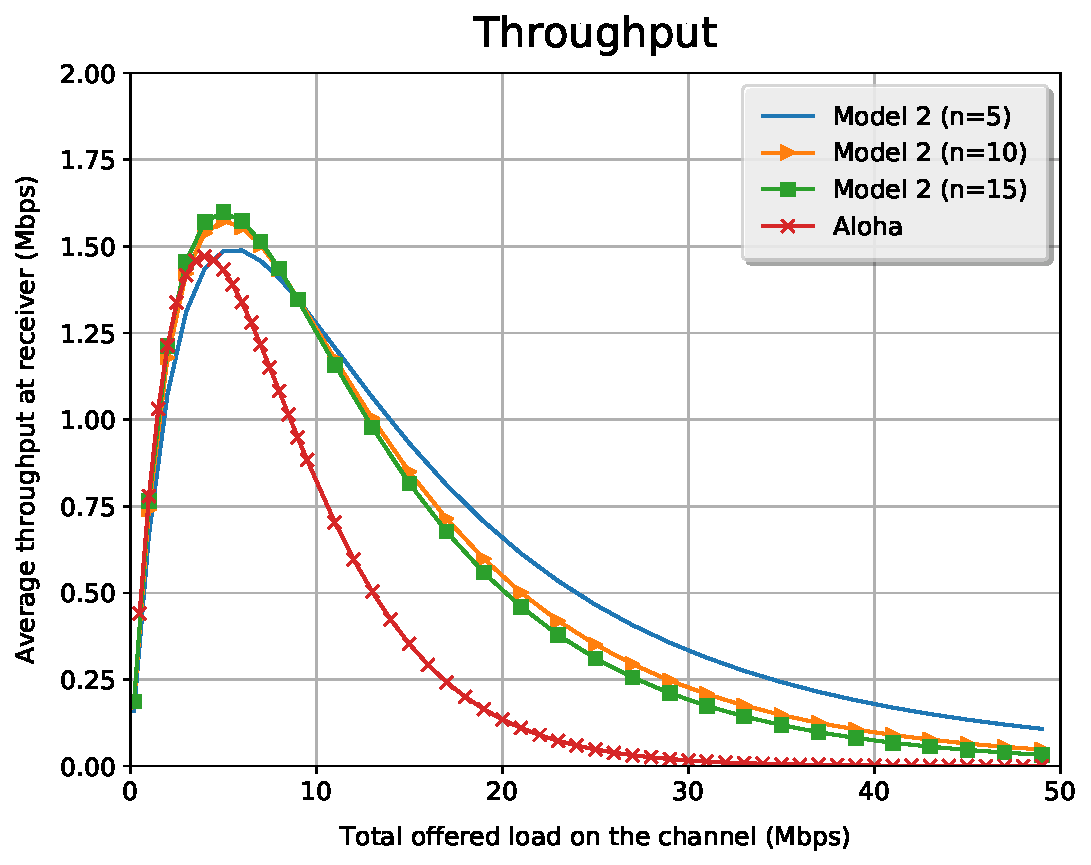
\includegraphics[width=.99\columnwidth]{figures/tr_1g1b}
	\caption{The plot shows the throughput predicted by the second model for different network sized.}
	\label{fig:tr_1g1b}
\end{figure}

\cref{fig:cr_10} shows the collision rate predicted by the different models.
The first model has a lower collision rate than the first one, that also justify the higher throughput.
The collision rate of the simulator at low loads is smaller than the second model, then gets slightly higher for medium and high loads.

\begin{figure}[t]
	\centering
	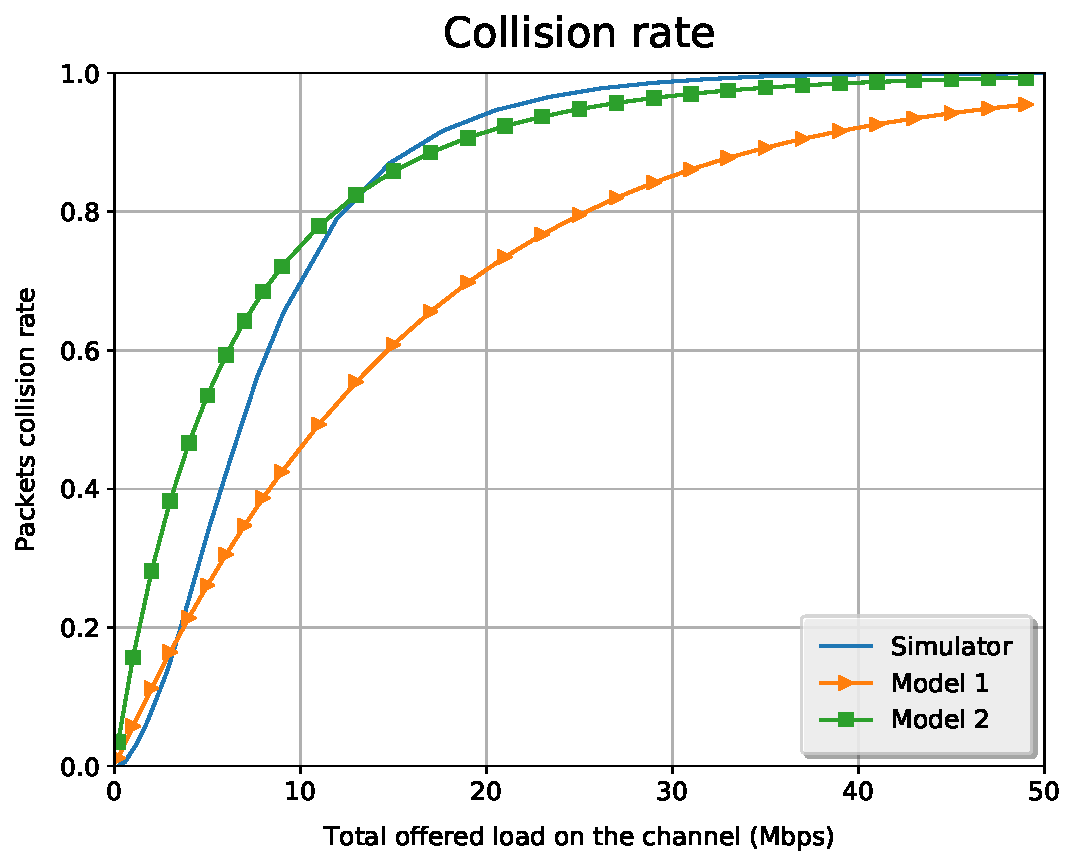
\includegraphics[width=.99\columnwidth]{figures/cr_10}
	\caption{The plot shows the collision rate predicted by the different for a network with 10 stations, compared with the simulator results.}
	\label{fig:cr_10}
\end{figure}


\section{Conclusion}
\label{sec:conclusion}

In this work, we built a Markovian model for the Aloha \ac{MAC} protocol.
We started from a quick overview of the protocol and the theoretical available model.
We build a very simple model based on a \ac{CTMC}, then we refined it to better represent the real behaviour of the system.
Finally, we compared the models with the simulator results.

The proposed model is able to predict the behaviour of Aloha in terms of throughput and packets collision rate for an arbitrary number of station and different transmission rates.
Our analysis shows that networks with a high number of stations achieve a slightly higher throughput at low load, but a considerably smaller one at high loads than networks with few nodes.
This is confirmed by the collision rate, low for small loads and very closed to $1$ for high loads.

Modelling a system is fundamental to get a good understanding of its behaviour and predict its evolution.
Models are cheap but give very useful indications.
Models should be used, together with simulators, in the design of each complex in order to achieve the desired goals with a high confidence.


\bibliographystyle{IEEEtran}
\bibliography{references}

\end{document}
